\documentclass[conference]{IEEEtran}

\usepackage{graphicx}
\usepackage{xcolor}
\usepackage{hyperref}
\usepackage{booktabs}
\usepackage{listings}
\usepackage{cite}
\usepackage{tikz}
\usetikzlibrary{positioning,arrows.meta,fit}

\definecolor{todocolor}{RGB}{192,0,0}
% Use \todoblock{label}{instructions} to mark a section that still needs
% real data from your own Wireshark captures. Search for "todoblock" and
% delete every occurrence before final submission.
\newcommand{\todoblock}[2]{%
  \par\noindent\textbf{\textcolor{todocolor}{[#1]}}~\textit{\textcolor{todocolor}{#2}}\par%
}

\lstset{
  basicstyle=\ttfamily\footnotesize,
  breaklines=true,
  columns=flexible,
  frame=single,
  framerule=0.3pt,
}

\begin{document}

\title{
  
\includegraphics[height=1.05cm]{figures/hsrw_logo.png}
  \hfill
  
\includegraphics[height=1.05cm]{figures/crl_logo.png}\\[10pt]
  Multi-Protocol Traffic Generation and Analysis:\\
  A Containerized System for HTTP/2, QUIC, MQTT and Raw TCP/UDP
}

\author{
  \IEEEauthorblockN{Amine Ahamri}
  \IEEEauthorblockA{
    Mobile \& Internet Computing\\
    Hochschule Rhein-Waal\\
  }
}

\maketitle

\begin{abstract}
This report describes a containerized system that generates and controls network
traffic across five protocols at once: HTTP/2, QUIC, MQTT and raw TCP/UDP. Ten
Docker containers are coordinated by a central controller that reads YAML traffic
profiles and steers four generators through a REST API. The system supports
constant, periodic-burst, linearly ramped and Poisson-distributed sending patterns,
an autonomous Adaptive Control loop that reacts to error rates and latency, and a
stealth mode for the TCP/UDP generator that hides its statistical fingerprint. This
report covers the architecture, the implementation decisions behind it, the
configuration format, and the Wireshark-based traffic analysis.
\end{abstract}

\begin{IEEEkeywords}
HTTP/2, QUIC, MQTT, Docker, traffic generation, Wireshark, behavioral fingerprinting, adaptive control
\end{IEEEkeywords}

\section{Introduction}

A normal office network never carries just one protocol. At any moment there is
web traffic, IoT sensor data, video calls and background sync jobs all sharing
the same wire. Studying how these protocols behave together, how they fail, and
how easy they are to tell apart from the outside, needs a testbed that can
actually produce that mix on demand and let you turn the dials while it runs.

This project builds exactly that testbed, based on the assignment in
\cite{hsrwassignment}. It generates traffic for five protocols at the same
time: HTTP/2 \cite{rfc7540}, QUIC/HTTP-3 \cite{rfc9000, rfc9114}, MQTT
\cite{mqtt5} with all three QoS levels, and raw TCP and UDP. Everything runs
as ten Docker containers orchestrated with Docker Compose \cite{dockercompose},
started with one \texttt{docker-compose up}. A central controller loads a YAML profile
and tells four traffic generators what to send and how fast; a web dashboard
lets you change any of that live, without restarting anything.

Beyond the basic rate and payload-size knobs, the system implements four
sending patterns (constant, periodic burst, linear ramp and Poisson-distributed
random intervals), a stealth mode that makes the raw TCP/UDP generator
statistically indistinguishable from normal traffic, and an autonomous Adaptive
Control loop that scales a generator's rate up or down based on the error rate
it is currently seeing, with no human in the loop.

The rest of this report is organized as follows. Section II describes the
architecture. Section III walks through the implementation decisions that
mattered, and why they were made that way. Section IV documents the
configuration format. Sections V through VII present the Wireshark-based
traffic analysis, the failure-visibility results and the single- versus
multi-machine comparison. Section VIII reflects on what the data actually
showed about protocol behavior, and Section IX documents how AI tools were
used while building this.

\section{System Architecture}

The system has ten containers on one Docker bridge network called
\texttt{mic-net}. Containers find each other by service name through Docker's
internal DNS, so \texttt{gen-http2} can simply call
\texttt{http://target-http2:8080} without anyone configuring an IP address
anywhere.

The ten containers fall into four groups. The \textbf{controller} (FastAPI,
port 8000) is the brain: it reads the YAML profile, drives the four generators
through their REST APIs and runs the Adaptive Control loop. The four
\textbf{generators} (\texttt{gen-http2}, \texttt{gen-quic}, \texttt{gen-mqtt},
\texttt{gen-tcpudp}) each keep their own state and expose the same four
endpoints: start, stop, patch the config, get the status. They are built on
\texttt{httpx} (HTTP/2), \texttt{aioquic} \cite{aioquic} (QUIC), \texttt{paho-mqtt}
\cite{pahomqtt} (MQTT) and plain Python sockets (raw TCP/UDP). The three
\textbf{target services} (\texttt{target-http2}, \texttt{target-quic},
\texttt{target-tcpudp}) plus the Mosquitto broker \cite{mosquitto} simply receive traffic and,
in two of the three cases, report what they received back to the metrics
collector. \texttt{target-http2} runs on Hypercorn \cite{hypercorn}, the only
ASGI server in the project that supports HTTP/2 natively. The \textbf{metrics collector} (Flask, port 9090) aggregates
everything into one \texttt{/metrics} response, and the \textbf{dashboard}
(a single static HTML file served over port 3000) polls the controller every
two seconds and renders the live state.

Fig.~\ref{fig:architecture} shows how a request actually travels through the
system. The dashboard never talks to a generator directly; every change goes
through the controller, which is what makes it possible to log every
configuration change with a timestamp, as the assignment requires.

\begin{figure*}[t]
\centering
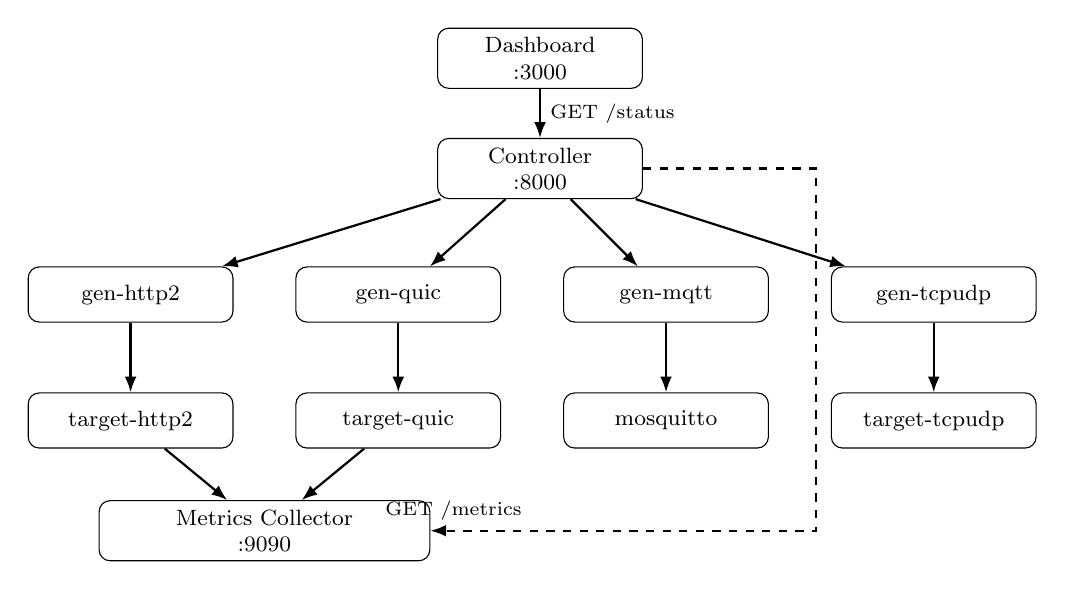
\begin{tikzpicture}[
  box/.style={draw, rounded corners, minimum width=2.6cm, minimum height=0.7cm, align=center, font=\footnotesize},
  arr/.style={-{Latex[length=2mm]}, thick},
  column sep/.style={column sep=1.1cm},
]
\node[box] (dash) at (5.2,6) {Dashboard\\:3000};
\node[box] (ctrl) at (5.2,4.6) {Controller\\:8000};

\node[box] (h2)     at (0,3) {gen-http2};
\node[box] (quic)   at (3.4,3) {gen-quic};
\node[box] (mqtt)   at (6.8,3) {gen-mqtt};
\node[box] (tcpudp) at (10.2,3) {gen-tcpudp};

\node[box] (th2)    at (0,1.4) {target-http2};
\node[box] (tquic)  at (3.4,1.4) {target-quic};
\node[box] (broker) at (6.8,1.4) {mosquitto};
\node[box] (ttcp)   at (10.2,1.4) {target-tcpudp};

\node[box, minimum width=4.2cm] (metrics) at (1.7,0) {Metrics Collector\\:9090};

\draw[arr] (dash) -- (ctrl) node[midway, right, font=\scriptsize] {GET /status};
\draw[arr] (ctrl) -- (h2);
\draw[arr] (ctrl) -- (quic);
\draw[arr] (ctrl) -- (mqtt);
\draw[arr] (ctrl) -- (tcpudp);
\draw[arr] (h2) -- (th2);
\draw[arr] (quic) -- (tquic);
\draw[arr] (mqtt) -- (broker);
\draw[arr] (tcpudp) -- (ttcp);
\draw[arr] (th2) -- (metrics);
\draw[arr] (tquic) -- (metrics);
\draw[arr, dashed] (ctrl.east) -- ++(2.2,0) |- node[pos=0.97, above, font=\scriptsize] {GET /metrics} (metrics.east);
\end{tikzpicture}
\caption{Component diagram of the single-machine deployment. Solid arrows are
REST calls or raw protocol traffic; the dashed arrow is the controller reading
aggregated metrics for status reporting and Adaptive Control.}
\label{fig:architecture}
\end{figure*}

One detail worth pointing out: \texttt{target-tcpudp} does not report to the
metrics collector at all, unlike the other two targets. It only accepts
connections and discards the data. This is deliberate, since the point of that
container is to make a TCP RST visible in Wireshark when it goes down, and
adding a reporting path would only get in the way of that.

\section{Implementation Decisions and Trade-offs}

\subsection{Connection reuse vs. a fresh connection per packet}

The HTTP/2 generator opens one \texttt{httpx} client with HTTP/2 enabled and
keeps it open for the whole run, firing several requests at once over that
single connection to actually use multiplexing rather than just claiming to.
The QUIC generator does the same thing for the same reason: a QUIC handshake
costs at least one extra round trip, and if the generator reconnected for
every request that handshake cost would swamp the latency numbers and make
QUIC look artificially slow next to HTTP/2 and MQTT, both of which also keep a
connection open.

The TCP/UDP generator does the opposite on purpose. For every single TCP
packet it opens a new connection, sends, and closes it again. This was not an
oversight. A fresh connect/close cycle produces a real SYN, SYN-ACK and FIN
sequence in the capture, which is exactly what is needed later for the
Failure Visibility analysis and for telling raw TCP apart from the
application-level protocols in a protocol hierarchy view.

\subsection{Mode and pattern as two separate knobs}

The TCP/UDP generator splits "what does a packet look like" from "how is it
paced over time". \texttt{mode} controls size and base interval: normal mode
uses a fixed 512 bytes every 100 ms, stealth mode draws a random size between
64 and 1400 bytes with Poisson-distributed timing. \texttt{pattern}
independently controls the sending cadence on top of that: constant, periodic
burst, or an extra random gap. Keeping these two orthogonal made it possible
to test, for example, stealth-mode sizing combined with a burst cadence, which
would not have been possible if mode and pattern were the same setting.

\subsection{The Poisson pattern on every protocol, not just one}

The assignment only asks for a random, Poisson-distributed pattern somewhere
in the system. This implementation puts it on all four generators using
\texttt{random.expovariate(1/interval)} (or NumPy's exponential distribution
for the TCP/UDP generator), which produces exponentially distributed gaps
between sends with the same average rate as the constant pattern. The reason
to extend it everywhere was to be able to show one single Wireshark capture
where HTTP/2, QUIC and MQTT all use Poisson timing at once, alongside TCP/UDP
stealth mode, rather than only ever demonstrating it on one protocol.

\subsection{Warmup and cooldown double as the ramp pattern}

Rather than building a separate "ramp" mode per protocol, the warmup and
cooldown periods are handled once, centrally, in the controller. A function
called \texttt{\_ramp\_rates()} steps every generator's rate field linearly
from zero up to its configured target over the warmup window, and back down
to zero over the cooldown window, sending the new value through the normal
PATCH endpoint at each step. This single mechanism satisfies both
requirements at once: the warmup/cooldown behavior the assignment asks for,
and the "ramping" sending pattern, since the gradual change shows up as a
slope in a Wireshark I/O graph either way.

\subsection{Adaptive Control}

The controller can run an autonomous control loop, either because a YAML
phase turns it on or because it was switched on manually. Every few seconds it
checks each generator's error rate, and where reported its latency, against
configurable thresholds, and scales the rate up or down by a multiplier
bounded on both ends. This goes past the baseline requirements, but it ties
directly into the resilience patterns covered in the course: the system reacts
to an injected failure on its own, without anyone touching a slider.

\section{Configuration Format}

The controller reads multi-phase YAML profiles from the \texttt{config/}
folder. Every profile has a \texttt{global} block with the total duration,
warmup and cooldown in seconds, and a list of \texttt{phases}. Each phase has
a name, a duration, an optional \texttt{adaptive\_control} block, and a
\texttt{protocols} block with one entry per protocol that should be active
during that phase. Three profiles ship with the project: \texttt{balanced.yaml}
(constant baseline, then stealth plus random pattern, then adaptive control),
\texttt{http2\_heavy.yaml} (HTTP/2 under load with a burst phase), and
\texttt{mqtt\_heavy.yaml} (a QoS 0 vs.\ QoS 2 vs.\ mixed comparison).

\begin{table}[t]
\centering
\caption{Per-protocol configuration fields}
\label{tab:config-fields}
\footnotesize
\begin{tabular}{@{}p{0.16\linewidth}p{0.78\linewidth}@{}}
\toprule
\textbf{Protocol} & \textbf{Fields} \\
\midrule
http2 & rate, payload\_size, method\_get\_pct, concurrent\_streams, get\_paths, post\_paths, pattern, burst\_rate, burst\_duration, burst\_interval, fault\_rate, extra\_latency\_ms \\
quic & rate, payload\_size, stream\_count, use\_0rtt, pattern, fault\_rate, extra\_latency\_ms \\
mqtt & rate, payload\_size, qos, topic\_count, qos\_distribution, pattern, fault\_rate, extra\_latency\_ms \\
tcp/udp & tcp\_rate, udp\_rate, packet\_size, mode, mean\_interval, min\_size, max\_size, tcp\_ratio, pattern, burst\_size, burst\_interval, fault\_rate, extra\_latency\_ms \\
\bottomrule
\end{tabular}
\end{table}

Field names in the YAML have to match the generator's Pydantic model exactly.
Anything that does not match is silently ignored rather than rejected, since
the models accept extra keys for forward compatibility but the generators only
apply the ones they actually recognize. One concrete example of this showing
up in the shipped profiles: a few phases list an explicit \texttt{topics}
array for readability, but the MQTT generator only ever looks at
\texttt{topic\_count}. The named list currently has no effect at runtime. This
is a known gap rather than something hidden, and it is worth fixing if there
is time left before submission.

Configuration is not locked to the YAML once the system is running.
\texttt{POST /config/load} switches the active profile and applies phase one
immediately if the system is already started. \texttt{PATCH /generator/\{name\}}
forwards any subset of the fields in Table~\ref{tab:config-fields} to one
generator. The dashboard wraps every one of these fields in a slider, toggle
or text input that calls the same two endpoints, debounced so that dragging a
slider does not flood the controller with requests.

\section{Traffic Analysis Results}

This section presents the five required Wireshark captures. Each subsection
below has the exact setup already filled in, since that part does not depend
on the actual capture, only on what to insert once the capture exists.

\subsection{Protocol Distribution}

Capture at least 60 seconds with the \texttt{balanced} profile running all
four generators. Export Statistics $\rightarrow$ Protocol Hierarchy as a
screenshot.

\todoblock{INSERT}{Screenshot of the Protocol Hierarchy and the percentage
breakdown of TCP vs.\ UDP, and within TCP the HTTP/2 (port 8080), MQTT (port
1883) and raw TCP shares, plus the UDP-only QUIC share (port 4433).}

\subsection{Temporal Analysis}

Capture 120 seconds with the \texttt{http2\_heavy} profile, which includes a
periodic-burst phase (burst rate 400 for 5 seconds every 30 seconds). Export
Statistics $\rightarrow$ I/O Graph with one line per protocol filter.

\todoblock{INSERT}{I/O graph screenshot with the burst peaks marked, plus a
second capture of a warmup period and a Random/Poisson phase for comparison
against the constant and burst shapes.}

\subsection{Behavioral Fingerprinting}

Capture two 30-second windows of the TCP/UDP generator alone: one in
\texttt{mode=normal}, one in \texttt{mode=stealth}. Optionally extend this with
the \texttt{balanced\_with\_stealth} phase, which runs stealth mode together
with the random pattern on HTTP/2, QUIC and MQTT at the same time.

\todoblock{INSERT}{Packet-length histograms and inter-arrival-time
distributions for both modes, with an explicit statement of which
characteristics are distinguishable (e.g.\ the fixed 100\,ms spacing in normal
mode) and which overlap with real client traffic.}

\subsection{Failure Visibility}

Capture across a \texttt{docker stop target-http2} event during normal
operation. Filter on \texttt{tcp.flags.reset==1} for the TCP RST, or look for
repeated SYNs to port 1883 if stopping \texttt{mosquitto} instead.

\todoblock{INSERT}{Measured time from the stop command to the first visible
failure indicator, and which protocol-specific signal appeared. See Section VI
for the deeper discussion of this capture together with the Adaptive Control
reaction.}

\subsection{Multi-System Deployment}

Capture on the physical network interface of either lab machine (not
\texttt{docker0}/\texttt{br-*}) while \texttt{docker-compose.targets.yml} runs
on Machine B and \texttt{docker-compose.generators.yml} runs on Machine A with
\texttt{TARGET\_B\_IP} pointing at Machine B.

\todoblock{INSERT}{Capture screenshot plus measured latency per protocol,
compared against an equivalent single-machine run. See Section VII for the
full comparison.}

\section{Failure Analysis Results}

\todoblock{INSERT}{Consolidated discussion of the Failure Visibility capture
from Section V-D. Cover: the per-protocol failure signal observed (TCP RST,
MQTT reconnect attempts, QUIC connection-close frames), how long it took to
become visible, and what the unaffected protocols looked like during the
outage. If Adaptive Control was enabled during the same run, add the
controller's logged decisions (error rate, multiplier, action) and how
quickly the affected generator's rate was scaled down and back up once the
target recovered.}

\section{Single-Machine vs. Multi-Machine Comparison}

\todoblock{INSERT}{Quantitative table: latency\_ms per protocol on a single
machine (loopback) vs.\ on two machines (real Ethernet hop). Add a short note
on what only becomes visible in the multi-machine capture: real host IP
addresses instead of Docker's 172.x.x.x range, no shared Docker bridge, and
genuine Ethernet framing under load.}

\section{Reflection on Protocol Behavior Under Different Traffic Patterns}

This section should pull together what Sections V through VII actually showed,
not repeat them. Questions worth answering once the data is there:

\begin{itemize}
\item Which protocol was easiest to fingerprint in normal, non-stealth
conditions, and why?
\item Did the random pattern change the I/O graph shape equally for every
protocol, or did some (HTTP/2 firing several streams per cycle, for instance)
keep some residual periodicity?
\item Did the measured packet-to-message ratio for MQTT match the expected 1x
for QoS 0 and 4x for QoS 2?
\item How did Adaptive Control's reaction time compare to the raw,
protocol-level failure detection time (TCP RST in under a second vs.\ the
configured check interval)?
\item What would change about distinguishability if TLS were used everywhere,
including MQTT and raw TCP?
\end{itemize}

\todoblock{INSERT}{Two to four paragraphs answering the points above with
concrete numbers from your own captures.}

\section{AI Usage Documentation}

I used Anthropic's Claude throughout this project, working directly in the
repository through an agentic coding session with file and shell access.

For the code, I used it to scaffold the first version of the
\texttt{docker-compose.yml} layout, the controller's FastAPI skeleton and the
four generators' REST contract (start, stop, patch config, get status), and
then iterated on that by hand and through more prompts. The Adaptive Control
loop, the warmup/cooldown ramp, the random pattern on all four generators and
the per-protocol fault injection were built the same way, one function at a
time, with a Python syntax check after every change. The OpenAPI/Swagger
documentation was generated from the Pydantic models and FastAPI decorators
and kept in sync with a small regeneration script run after every API change.

For the documentation, I had it review the README and the docs against the
actual code and fix what no longer matched, for example an old claim that the
TCP/UDP generator used Scapy when the real implementation just uses plain
sockets.

This report itself was drafted the same way: the architecture, implementation
and configuration sections came from the verified source code, while the
traffic analysis, failure analysis and multi-machine sections were left as
placeholders on purpose, since those need real Wireshark captures that only I
can produce on lab hardware.

I reviewed every change before accepting it and ran the syntax checks myself.
I also went through the entire codebase module by module in a separate
walkthrough session to make sure I could explain every part of it on my own,
not just recognize that it works.

\todoblock{INSERT}{Replace this paragraph with your own honest account before
submission, including anything I missed above.}


\bibliographystyle{IEEEtran}
\bibliography{references}

\end{document}
